\documentclass{standalone}



\graphicspath{{img/Chap1}}

\begin{document}
\chapter*{Introduction}\addcontentsline{toc}{chapter}{Introduction}
\markboth{Introduction}{Introduction}
Sickle Cell Disease (SCD) is a group of inherited red blood cell disorders. A subject affected by SCD has abnormal hemoglobin, which causes the red blood cells to become hard and sticky and look like a sickle. Those cells die early, which causes a constant deficiency of red blood cells \cite{SickleCell}.

The main symptom of SCD is anaemia, a medical condition that consists in a low value of the haemoglobin (the substance that resides in the red blood cells, responsible of the oxygen transport) in blood.
Another frequent symptom is the occurrence of painful episodes known as \textit{sickle cell crisis} due to blood vessels that become blocked and are frequently localized in limbs or back.
People with SCD are more vulnerable to infections, particularly in the early ages of life \cite{SickleCell_symptoms}.

The most common neurological complication in subjects with SCD is the presence of Silent Cerebral Infarcts (SCIs)\cite{ART:Pegelow}.
SCIs are defined as an abnormal magnetic resonance imaging of the brain in the setting of a normal neurologic examination, without a history or physical findings associated with an overt stroke \cite{ART:Debaun}.
In the brain magnetic resonance imaging(MRI) SCI usually present itself as an hypointense region in the T-1 weighted image, or as an hyperintense region in the FLAIR image, and are localized in the white matter as show in \figurename~\ref{fig:HealthVSLesion}.


\begin{figure}[h!]
		\centering
        \begin{subfigure}[b]{0.45\textwidth}
             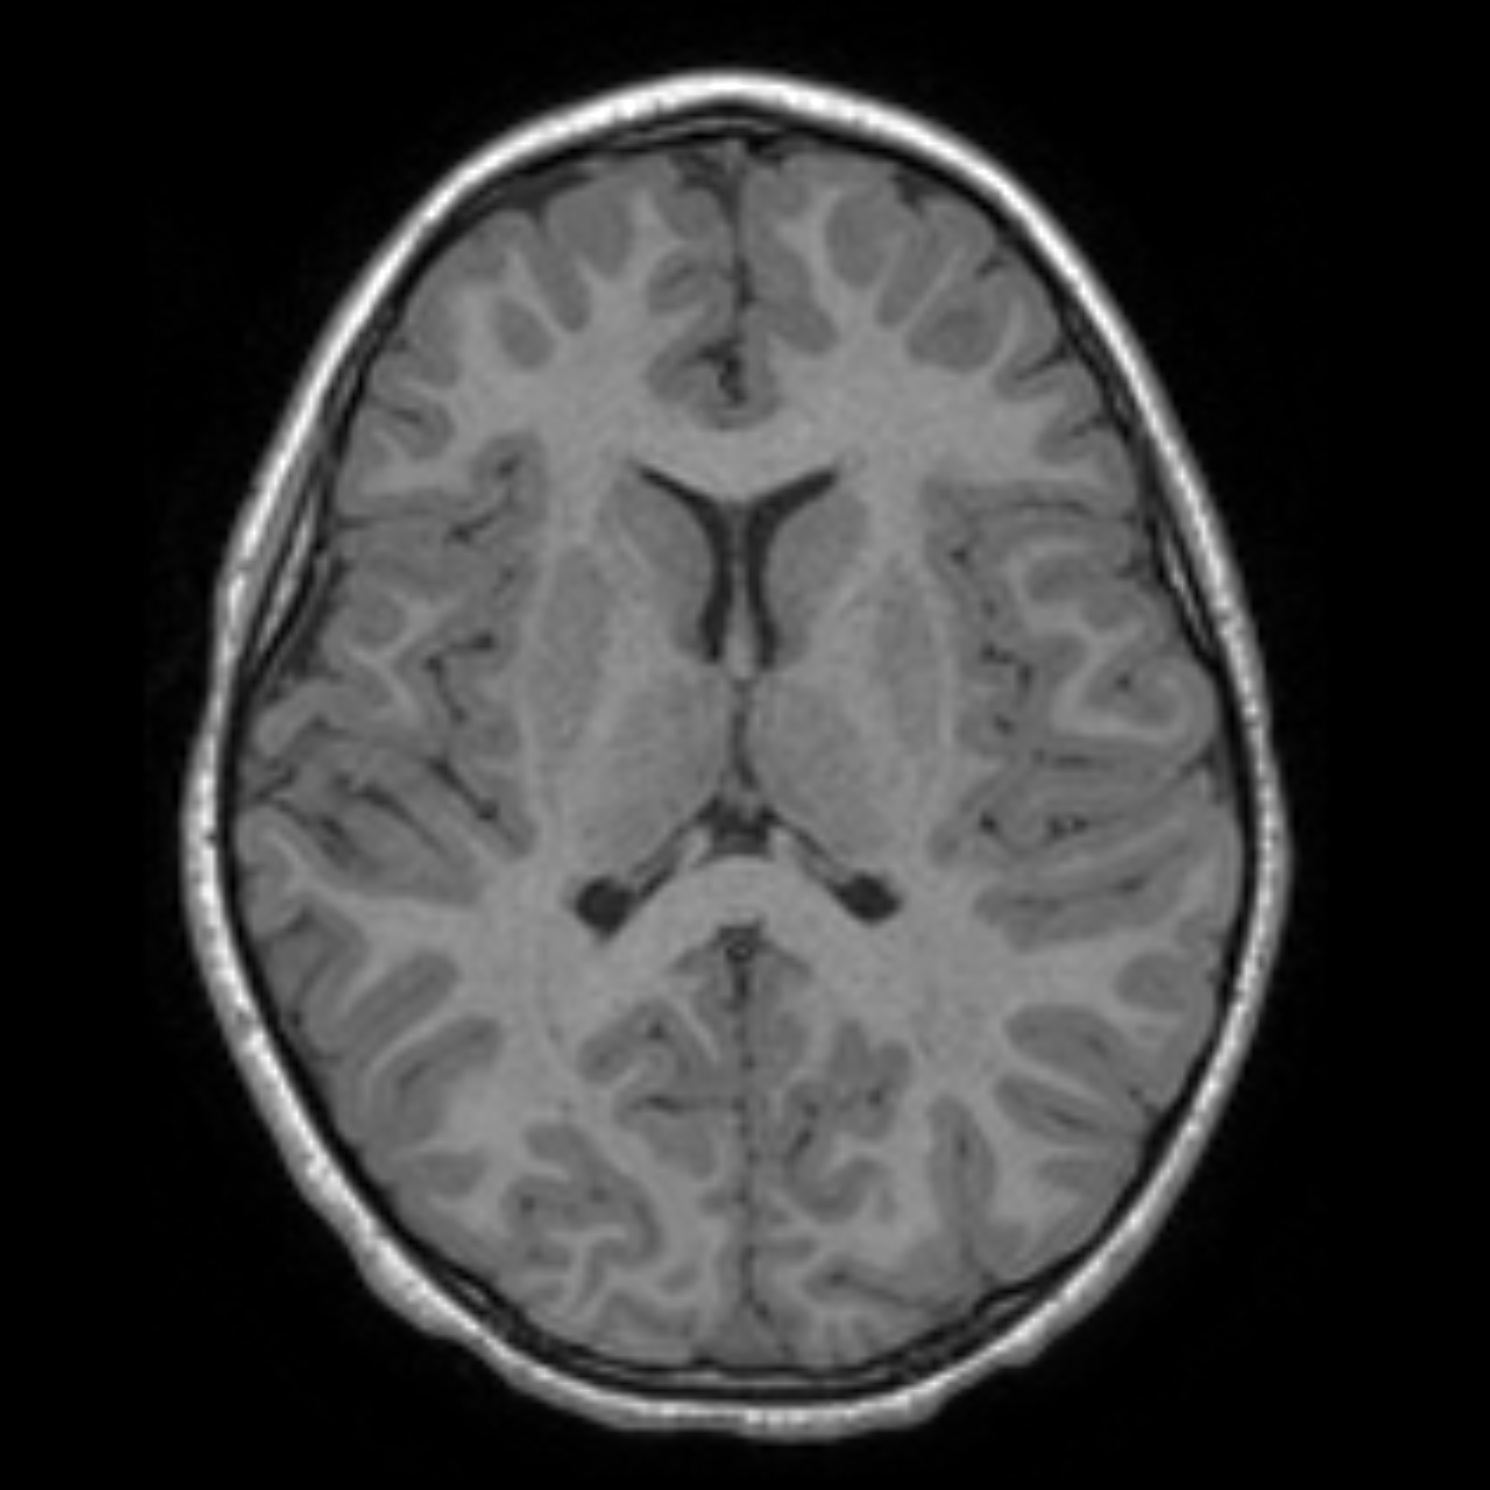
\includegraphics[scale=0.13]{img/Chap1/Normal_T1.png}
             \caption{Axial slice of a T1-weighted MR scan without SCI evidences}
             \label{fig:Normal_T1}
        \end{subfigure}
        \hfill
        \begin{subfigure}[b]{0.45\textwidth}
             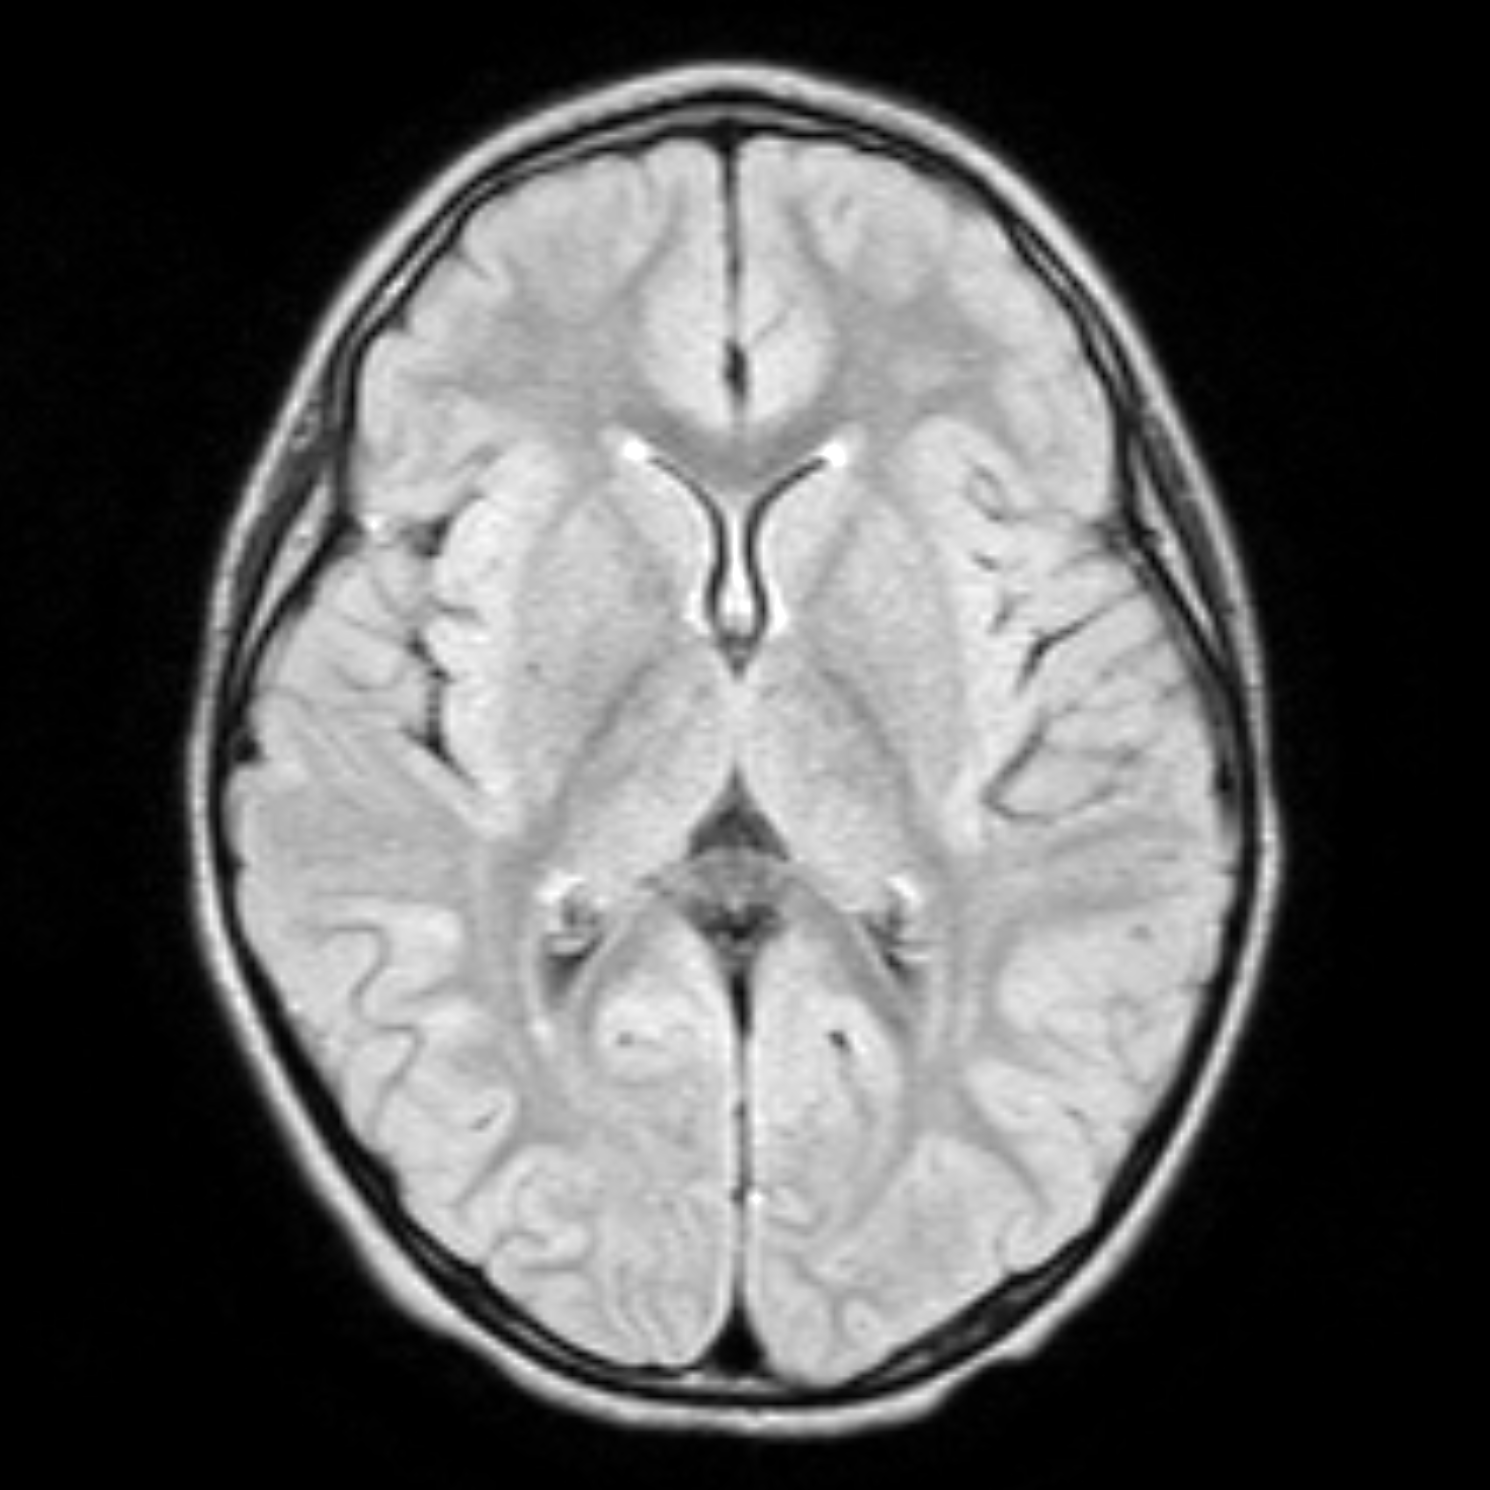
\includegraphics[scale=0.13]{img/Chap1/Normal_flair.png}
             \caption{Axial slice of a FLAIR MR scan without SCI evidences}
             \label{fig:Normal_flair}
        \end{subfigure}
        \hfill
        \vfill
        \begin{subfigure}[b]{0.45\textwidth}
             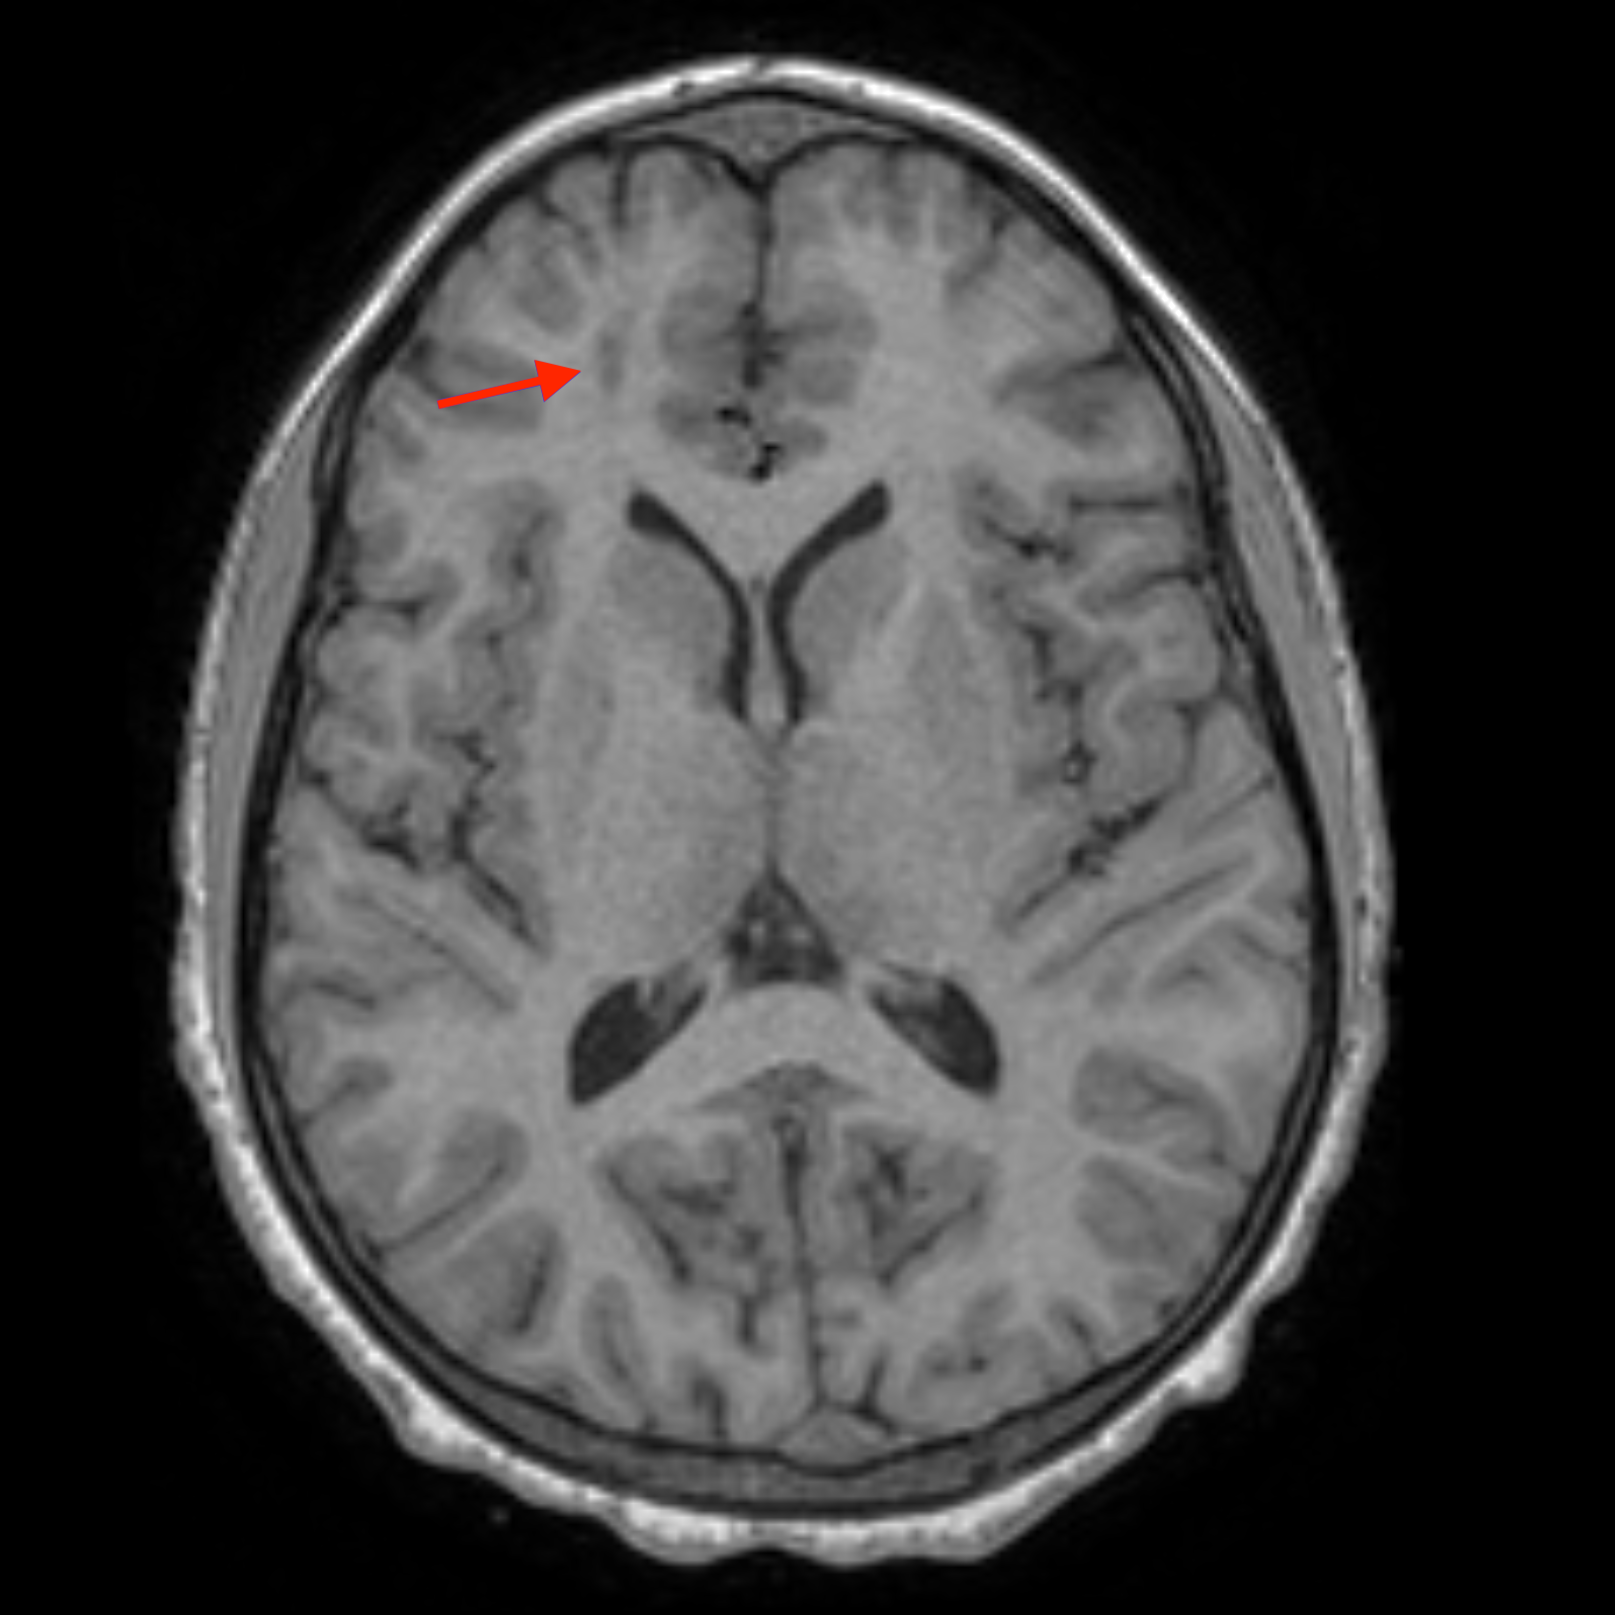
\includegraphics[scale=0.12]{img/Chap1/Lesion_T1.png}
             \caption{Axial slice of a T1-weighted MR scan with SCI evidences}
             \label{fig:SCI_T1}
        \end{subfigure}
        \hfill
        \begin{subfigure}[b]{0.45\textwidth}
             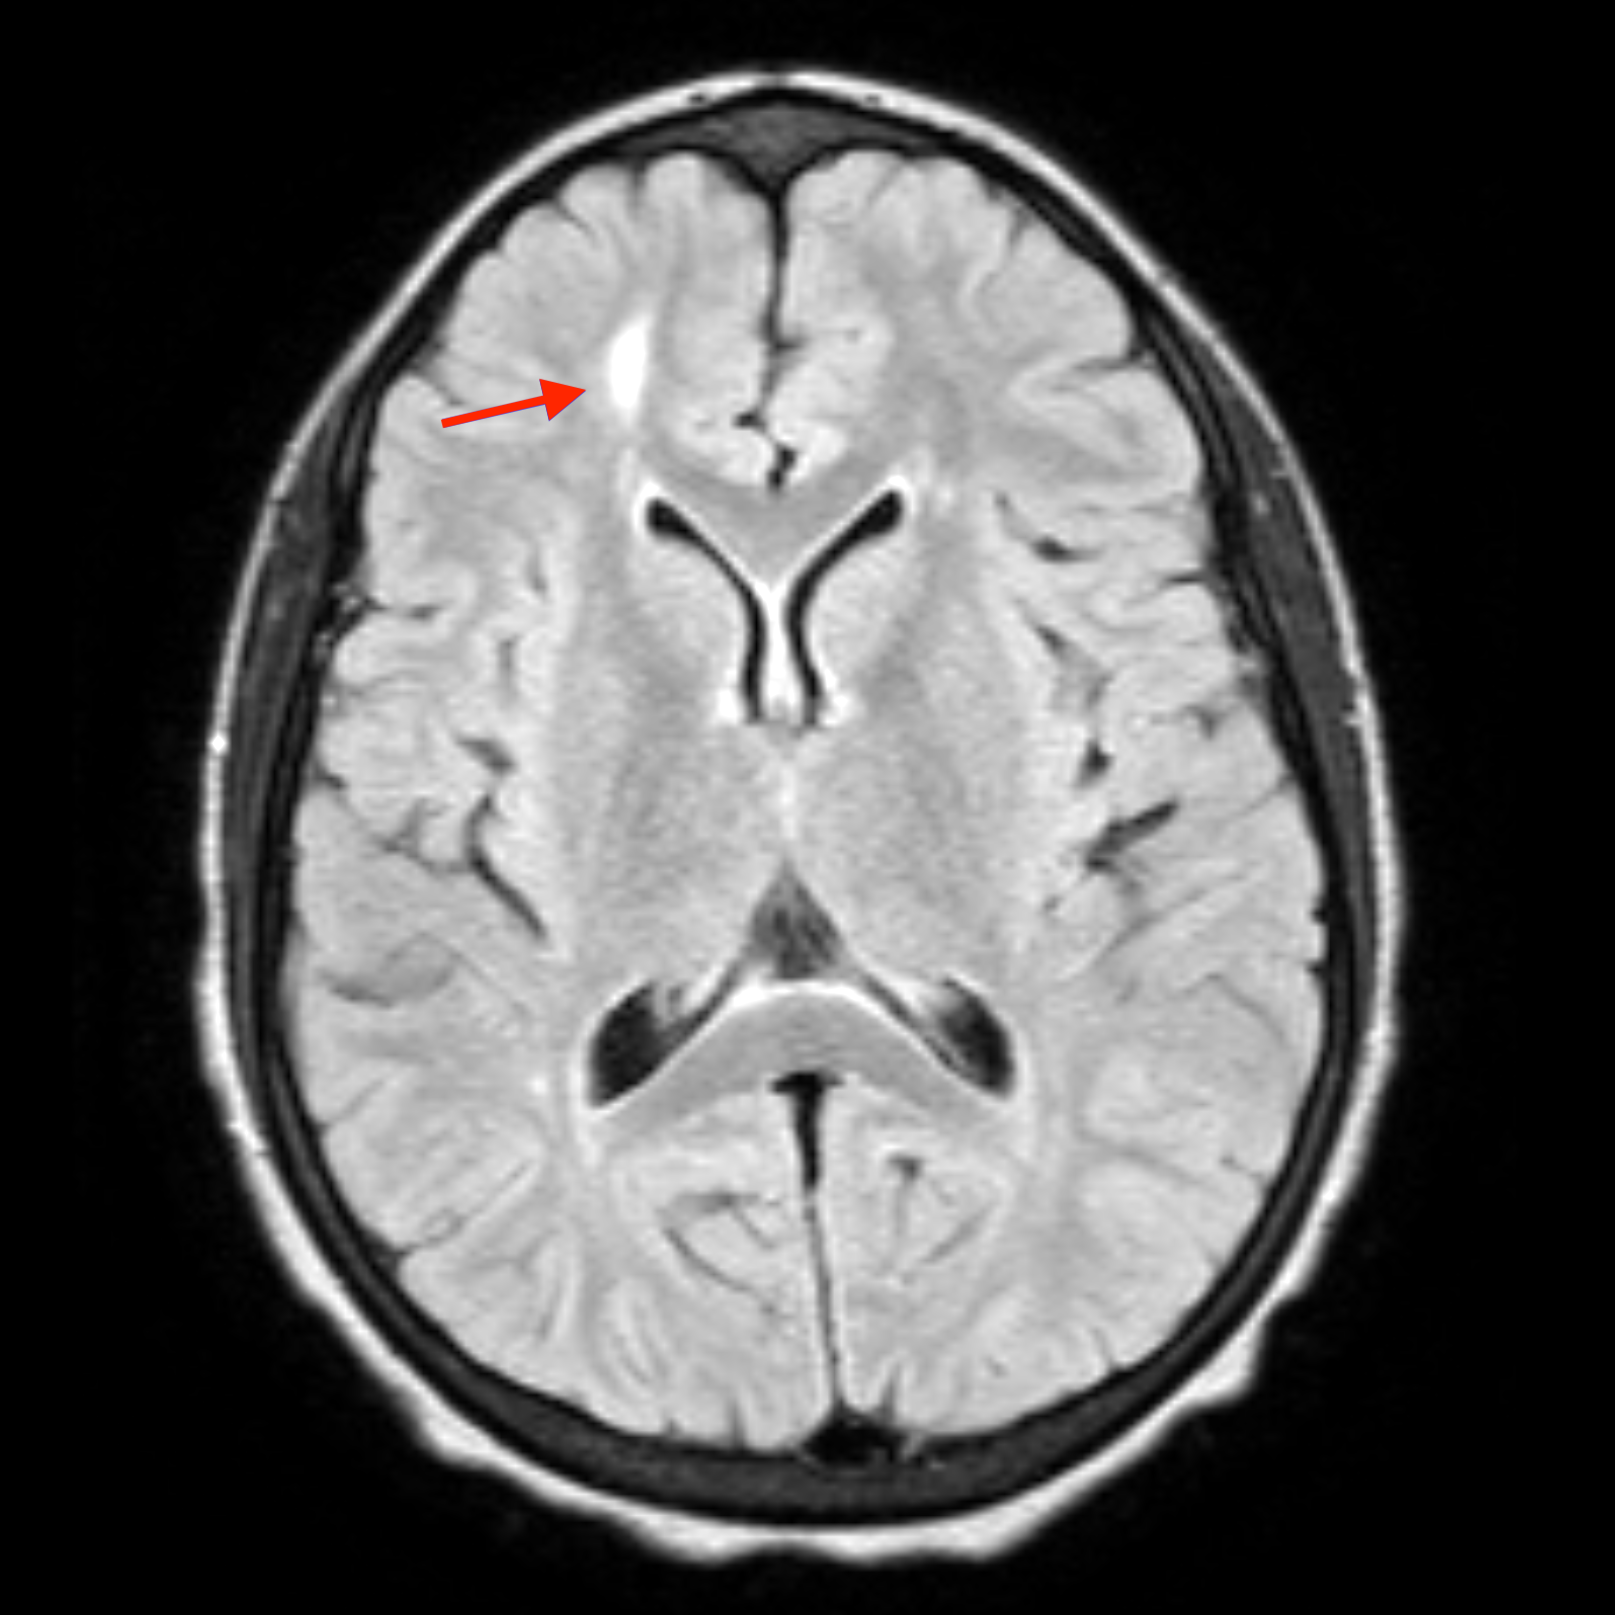
\includegraphics[scale=0.12]{img/Chap1/Lesion_flair.png}
             \caption{Axial slice of a FLAIR MR scan with SCI evidences}
             \label{fig:SCI_flair}
        \end{subfigure}
		\caption{Comparison between healthy brain image and brain with SCI in both T1-weighted and FLAIR MR scan. It's possibile to appreciate how the SCI appears as an hyperintense region in the FLAIR image and as an hypointense region in the T1-w image, pointed by the red arrow.}
		\label{fig:HealthVSLesion}
	\end{figure} 


SCIs' consequences includes a decrement in general intellectual abilities, poor academic achievement, working abilities and a minor quality of life \cite{ART:Debaun}. Specific morbidity can lead to a progression to overt stroke and progressive SCIs \cite{ART:Debaun, ART:Biondini}.
Neuropsychological and neuroimaging studies are needed to understand how SCI negatively affect cognition and provide a starting point for the identification of potential targets for preventive therapies \cite{ART:Howing}.
Up to now the segmentation of those lesions is manually made by high trained and specialized neuroradiologists, which is highly time consuming(severaly hours) and can be very subjectively, influenced by the experience of the operator.


To overcome those issues it was proposed the usage of a neural network to automatically segment the SCI in a brain MRI. 
A stepwise procedure was used to achieve the segmentation of those lesions, differentiating the segmented regions from other non-clinically relevant hypo regions in the white matter \cite{ART:Biondini}.

To do that it was necessary to process the MRI images before (pre-processing) and after (post-processing) the application of the implemented SCI segmentation tool.
In the pre-processing stage the aim is to prepare the image to be processed by the segmentation tool, cleaning it from everything could badly influence the success of the AI segmentation.
In the post-processing stage the purpose was to refine the results obtained by the neural network.

This work of thesis, made in collaboration with the Department of Neuroscience of the University of Padova, fits in the contest of the European project "Genomed4All"\cite{Genomed4All} which aims to find correlation between -omics data and phenotype by the help of Artificial Intelligence \cite{Humanitas} using European data of patients affected by haematologic diseases, that often presents anomalies in the DNA.

The purpose of this work of thesis is to develop reliable, open source and relatively quick strategies for the pre-processing and post-processing phase.



%TODO: Parlare di cosa sarà detto nei vari capitoli


\end{document}